% Convergence check (Step 0, synthetic data): report. Compile with tectonic, xelatex or pdflatex.
\documentclass[10pt,a4paper]{article}
\usepackage[a4paper,top=16mm,bottom=17mm,left=17mm,right=17mm]{geometry}
\usepackage[T1]{fontenc}
\usepackage{sourceserifpro}
\usepackage{sourcesanspro}
\usepackage{amsmath,amssymb}
\usepackage[table]{xcolor}
\usepackage{booktabs,tabularx,xltabular,array,float,graphicx}
\usepackage{enumitem}
\usepackage{caption}
\usepackage{titlesec}
\usepackage[most]{tcolorbox}
\usepackage{microtype}
\usepackage{needspace,etoolbox}
\pretocmd{\section}{\needspace{8\baselineskip}}{}{}
\usepackage[hidelinks]{hyperref}

\definecolor{ink}{HTML}{16212A}
\definecolor{muted}{HTML}{4F5E68}
\definecolor{rule}{HTML}{C9D3D8}
\definecolor{acc}{HTML}{0B6E69}
\definecolor{accs}{HTML}{EEF6F5}
\definecolor{warn}{HTML}{9A5B00}
\definecolor{warns}{HTML}{FBEFDC}
\definecolor{headbg}{HTML}{F1F5F6}

\setlength{\parindent}{0pt}
\setlength{\parskip}{4pt}
\linespread{1.04}
\titleformat{\section}{\sffamily\large\bfseries\color{acc}}{\thesection.}{0.5em}{}[{\color{rule}\titlerule}]
\titlespacing*{\section}{0pt}{10pt}{4pt}
\captionsetup{font={small,sf},labelfont={bf,sf},skip=3pt}
\setlist{itemsep=1pt,topsep=2pt,parsep=0pt,leftmargin=13pt}
\newcolumntype{L}{>{\raggedright\arraybackslash}X}
\newcolumntype{C}{>{\centering\arraybackslash}m{1.25cm}}
\newcolumntype{P}[1]{>{\raggedright\arraybackslash}m{#1}}
\renewcommand{\tabularxcolumn}[1]{m{#1}}
\renewcommand{\arraystretch}{1.16}
\newcommand{\pass}{{\sffamily\bfseries\color{acc}PASS}}
\newcommand{\note}{{\sffamily\bfseries\color{warn}PASS*}}
\newcommand{\hdr}[1]{\textsf{\textbf{#1}}}
\newtcolorbox{goodbox}{enhanced,colback=accs,colframe=acc,boxrule=0pt,leftrule=2.5pt,
  arc=0pt,left=7pt,right=7pt,top=5pt,bottom=5pt}
\newtcolorbox{warnbox}{enhanced,colback=warns,colframe=warn,boxrule=0pt,leftrule=2.5pt,
  arc=0pt,left=7pt,right=7pt,top=4pt,bottom=4pt,fontupper=\small}

\begin{document}
{\sffamily\bfseries\LARGE\color{ink} Convergence check on synthetic data\par}
\vspace{2pt}
{\sffamily\color{muted} Step 0 (convergence demo on synthetic data) of the method documentation\par}
\vspace{6pt}

\begin{goodbox}
{\sffamily\bfseries\large\color{acc} Verdict: ready to start the implementation in the emulator.}\par\smallskip
This check asked one question: if the proposed model is trained with meta-RL (PPO) as the documentation describes, does the
training actually work, and does it settle on a good policy? The answer is \textbf{yes}, once five small training changes are made
(Section~\ref{sec:changes}). Each change was tried and tested here. All 37 automatic pass/fail
criteria meet their targets; two of them (the KL rule in Stages A and B) carry a small note (Section~\ref{sec:results}). In short:
\begin{itemize}
\item \textbf{Training is stable.} Three runs started from different random seeds end at almost the same result in every stage.
\item \textbf{Decisions are near-optimal.} Where the best decision can be found by trying every option, the model matches it in 99.4\% of cases.
\item \textbf{It beats every comparison policy}, even one that is secretly told the true server speeds. This holds on a fixed system, on new random systems and under four kinds of changed conditions.
\item \textbf{It learns from its history.} It uses the results of past requests to discover servers that are secretly slow, and the gain is statistically clear on every seed.
\item \textbf{It is safe and fast.} It never breaks a hard rule (0 violations in 597\,000 checked decisions) and takes about 1--2\,ms per decision.
\end{itemize}
Three follow-up items move to the emulator stage (Section~\ref{sec:open}); none of them blocks the implementation.
\end{goodbox}

\section{Key terms in plain words}\label{sec:terms}
Standard reinforcement-learning terms (PPO, critic, entropy, KL, discount, GAE) are used as usual. The other terms of
this report mean the following.
\begin{itemize}
\item \textbf{Request, server, copy.} A user sends a request (for example, speech recognition). The scheduler may send it to one server or to several servers at once; each of these is a \emph{copy}. The first copy to finish is used and the others are cancelled. More copies lower the chance of being late but use more server time.
\item \textbf{Deadlines and reward.} Each request has a soft deadline $D^1$ and a hard deadline $D^2$. A request scores 1 if it finishes by $D^1$; the score then falls linearly to 0 at $D^2$, and a penalty is added after $D^2$. A small cost is subtracted for the server time all its copies used.
\item \textbf{Proposed model.} The decision model. At each decision it reads a set of \emph{tokens}: the waiting requests, the servers, the copies currently running and the history (results of recent finished copies). It then picks (request, server) pairs one by one until it chooses \emph{STOP}.
\item \textbf{Hidden speeds.} The model is never told how fast a server is. It must infer this from what it sees, mainly from the history.
\item \textbf{Hard rules (masks).} Rules the model cannot break: never exceed a server's capacity or the copy limit $d_{\max}$; always send a request that is about to miss its hard deadline; and if a server is idle and some request can be sent, send at least one copy (the model cannot simply do nothing). Other requests may still be held back to be sent later.
\item \textbf{Baseline.} A simple policy used for comparison. A \emph{privileged} baseline is given information the model does not have (here, the true speeds).
\item \textbf{Seed.} A training run with a different random start. If three seeds agree, the result is not luck.
\item \textbf{Twin systems and paired intervals.} Two systems that are identical except that one server is $3\times$ slower in one of them. Comparing results on twins removes all other randomness. A 95\% bootstrap interval that lies entirely above zero means the improvement is real and not noise.
\item \textbf{Open loop and closed loop.} These describe how requests reach the system. They matter for one question: how can the model notice a server that is secretly slow?
\begin{itemize}
\item \emph{Open loop} (realistic traffic). Users send requests whenever they want, so many requests are in progress at the same time and queues form. Picture a supermarket with several checkout counters and a steady stream of customers: if one cashier is slow, this is visible \emph{right now}, because that counter has a longer line and its customers have been waiting longer. In the same way, the model sees every copy that is currently running and how long it has been running, so it can spot a slow server from the present state alone, without remembering anything.
\item \emph{Closed loop} (artificial test). A new request is sent only after the previous one has finished, so every server is idle at every decision. In the supermarket picture, only one customer is in the shop at a time and every counter is always empty, so looking at the counters tells nothing. The only way to know that a cashier is slow is to \emph{remember} that the last few customers sent there took a long time. For the model, this memory is the history (the results of earlier requests). The name comes from the loop being ``closed'': each new request waits for the previous result to come back.
\end{itemize}
Why both are needed: in open loop, a model \emph{without} history can still find the slow server from the live queues, so comparing models with and without history there proves nothing. Closed loop removes this live clue, so any gain from history must come from actually using it.
\item \textbf{Stages (training setups).} A, B and C are three training setups, from easy to hard: A (one request at a time on a small fixed system), B (one fixed 5-server system with realistic traffic) and C (a new random system with hidden speeds in every episode, i.e.\ meta-RL). In this check each stage was trained separately, from scratch, to see whether training converges at that level of difficulty. Each trained model was then tested (inference only, no learning) on its own set of unseen systems. Stages do not exist at inference time: a deployed model simply receives requests and decides. The model to deploy is the Stage C one, since only it learned to handle unknown systems. Test H is a separate test, described in Section~\ref{sec:data}.
\end{itemize}

\section{What was used, and the synthetic data}\label{sec:data}
\textbf{Code and computer.} Everything was written from scratch in the folder \texttt{Convergence\_Check}:
the simulator, the systems, the model, PPO, the baselines and the evaluation. No code or data from the existing
project folders was used. All runs were on one laptop, inside a Python virtual environment (PyTorch 2.15).
Simulation ran on the CPU (12 threads), and the PPO training steps for Stages B and C ran on the laptop GPU (RTX 4050,
6\,GB). Memory use was limited so the laptop could not crash: at most 4 training runs at a time, at most 4\,GB per
evaluation, and a watchdog.

\textbf{The simulator} follows the model in the documentation. 12 unit tests check it.
\begin{itemize}
\item \textbf{Servers.} There are GPU-like and CPU-like servers. Each server has a speed and 3--5 slots. For each service it also has a chance of a slow outlier, which takes $5\times$ as long. Run times also vary randomly (log-normal noise, $\sigma=0.15$).
\item \textbf{Sharing a server.} When $n$ copies run on the same server, each one slows down: it runs at rate $1/(\text{base}\cdot(1+0.4(n-1)))$.
\item \textbf{Network.} Each user--server pair has a network delay drawn uniformly between 14 and 26\,ms, plus 1.5\,ms random jitter.
\item \textbf{Reward.} $r=P(T)-1.0\cdot\text{lateness}/D^2-0.1\cdot\text{busy time}/D^2$, where $P(T)$ is the score described in Section~\ref{sec:terms}.
\item \textbf{Services.} There are three made-up services: speech-like (with up to 15\% slow outliers on GPUs), detect-like and segment-like. Input sizes vary from $0.5\times$ to $2\times$. $D^1$ is 35--60\,ms and $D^2$ is 150\,ms.
\end{itemize}

\textbf{Synthetic systems and test sets.} Every test set is fixed, never seen in training, and the same for every policy.
\begin{itemize}
\item \textbf{Stage A.} One fixed system (2 GPU-like and 2 CPU-like servers), one request at a time, all servers idle. The test has 320 requests. For each one, all 15 possible server groups were tried by brute force (4000 random samples each) to find the best choice. This includes the group of all 4 servers, which the model is not allowed to pick (at most 3 copies), so the comparison is, if anything, strict.
\item \textbf{Stage B.} One fixed system of 5 servers. Requests arrive at random times at low, medium and high load (0.3, 0.6 and 0.85), and also in bursts (load 0.6, with bursts at $3\times$ the calm rate). The test has 12 episodes of 150 requests per load.
\item \textbf{Stage C (meta-RL).} Every episode is a new random system: 3--6 servers (1--2 GPU-like), speeds drawn uniformly between 0.6 and 1.4, and random capacities, outlier rates and loads; 30\% of episodes are bursty. Speeds are \emph{never} given to the model, and in half of the systems one GPU-like server is secretly $3\times$ slower. The test has 48 new systems, plus 24 twin pairs.
\item \textbf{History test H} (\emph{not} a stage of the method). A special test created only for this check: a separate model was trained and tested just to prove that the proposed model can learn from its history. It runs in closed loop (Section~\ref{sec:terms}) with only one copy allowed per request ($d_{\max}=1$), so the history is the only way to tell which server is slow. Two versions are trained, one with and one without history, and compared on the same systems. The test has 32 twin pairs of 96 requests each.
\item \textbf{Changed conditions (generalisation).} Larger systems (7--8 servers, 2--3 GPU-like, 40 users), overload (load 0.9--1.0), deadlines cut to $0.7\times$, and a traffic mix that is 70\% speech-like. Each condition has 32 systems.
\end{itemize}

\textbf{Baselines} (comparison policies).
\begin{itemize}
\item \textbf{Random-1:} sends each request to one random server.
\item \textbf{Redundancy-2:} sends each request to two random servers.
\item \textbf{JSQ:} sends each request to the server with the shortest queue.
\item \textbf{Greedy-Predict (privileged):} is told the true speeds, the secret slowdown and the outlier rates. It uses them to simulate each option and picks the best single server, or the best two of the top three.
\end{itemize}

\textbf{Model and training settings} (the configuration that passed the check).
\begin{itemize}
\item \textbf{Model.} The proposed model as documented, with the hard-rule masks. Size: width $d=64$, 2 layers, 4 attention heads. It sees at most $K=8$ waiting requests and $M=32$ history entries, and sends at most $d_{\max}=3$ copies per request.
\item \textbf{PPO.} 16 episodes per iteration, 4 epochs, minibatch 256, clip 0.2, entropy weight 0.01, target KL 0.02, $\gamma=0.99$ per time unit $\Delta$, and $\lambda=0.9$. Because decisions happen at irregular times, the discount is applied per elapsed time: a reward that comes $t$\,ms later counts with weight $\gamma^{t/\Delta}$, so each decision effectively looks about $100\,\Delta$ ahead. $\Delta$ is used only in training.
\item \textbf{Length of training.} Each PPO iteration collects 16 complete episodes, so training is measured in thousands of episodes: 4\,800 for Stage A, 6\,400 for B and C, and 3\,200 for H, per seed (Table~\ref{tab:volume}).
\item \textbf{Reporting.} Every result uses 3 seeds and the model at the end of training. No ``best'' checkpoint is hand-picked.
\end{itemize}

\begin{table}[H]
\centering\small
\caption{Training volume per seed. Times are wall-clock on the laptop, with up to 4 runs in parallel.}\label{tab:volume}
\begin{tabularx}{\textwidth}{@{}l r r L r r@{}}
\toprule
\hdr{Stage} & \hdr{PPO iterations} & \hdr{Episodes} & \hdr{One episode is} & \hdr{Requests} & \hdr{Time}\\\midrule
A & 300 & 4\,800 & 64 requests on the fixed 4-server system & 307\,200 & 43--48 min\\
B & 400 & 6\,400 & 150 requests on the fixed 5-server system, at a random load (30\% bursty) & 960\,000 & 37--39 min\\
C & 400 & 6\,400 & 150 requests on a \emph{new} random system, so 6\,400 different systems are seen & 960\,000 & 33--36 min\\
H & 200 & 3\,200 & 64 requests in closed loop on a new random system & 204\,800 & about 9 min\\
\bottomrule
\end{tabularx}
\end{table}

\clearpage
\section{Checks, how they were done, and results}\label{sec:results}
Each row below is one check. ``Status'' is PASS when the documented target is met on all three seeds.

\begingroup\small
\setlength{\LTpre}{2pt}\setlength{\LTpost}{2pt}
\begin{xltabular}{\textwidth}{@{}P{3.3cm}LL C@{}}
\toprule
\hdr{Check} & \hdr{How it was tested} & \hdr{Result (3 seeds, end of training)} & \hdr{Status}\\\midrule
\endfirsthead
\toprule
\hdr{Check} & \hdr{How it was tested} & \hdr{Result (3 seeds, end of training)} & \hdr{Status}\\\midrule
\endhead
The simulator is correct & 12 unit tests against the documented model (delays, server sharing, cancelling copies, reward, noise, load, twins, repeatability, rule audit) & 12 of 12 pass & \pass\\
Training converges (A, B, C, H) & The documented criteria on the training logs: the reward rises and then flattens; seeds end within 10\% of each other; the critic's explained variance rises; entropy falls but does not collapse too early; KL stays small & All criteria met in every stage. Spread of the final reward across seeds: A 0.3\%, B 4.0\%, C 8.7\%, H 0.8\%. Critic explained variance: 0.84--0.88 (B, C) and 0.55 (H). In A it is 0.09--0.11, which is 75--93\% of the highest value possible there (0.12). Median KL 0.005--0.023. Measured in episodes, the validation reward reaches 95\% of its total gain after about 340--660 training episodes (A), 2\,400--3\,400 (B), 340--500 (C) and 340--1\,140 (H), out of 4\,800 / 6\,400 / 6\,400 / 3\,200, and stays flat afterwards (Figure~\ref{fig:training}) & \note\\
Stage A: best decisions & The model's chosen server group vs the brute-force best of all 15 groups & 99.4\% of decisions within 1\% of the best, on every seed (target: at least 95\%). For comparison: untrained model 37.5\%, JSQ 31.9\%, privileged Greedy 99.1\% & \pass\\
Stage B: beats the baselines & Mean reward on the fixed test episodes at 4 loads & Every seed beats every baseline at every load, \emph{even privileged Greedy}: low load 0.91--0.93 vs 0.89, medium 0.68--0.75 vs 0.53, high 0.27--0.34 vs 0.21, bursty 0.59--0.65 vs 0.44 & \pass\\
Stage B: fewer copies when busy & Copies per request at low vs high load (sanity scenario 3 of the documentation) & 1.8--2.6 copies at low load vs 1.2--1.4 at high load: the model learned to save server time when servers are busy & \pass\\
Stage C: new random systems & 48 systems never seen in training, speeds hidden & Reward 0.42--0.47, vs 0.32 for privileged Greedy, 0.16 for Redundancy-2 and 0.07 for JSQ. 95th-percentile latency $1.7$--$1.9\times D^2$ vs $3.0\times$ for Greedy & \pass\\
History is used (test H) & On the same systems: reward of the model with history minus the model without history, with a 95\% paired interval & Gain of +0.013 to +0.018, interval above 0 on every seed. On slowed twins the model reaches 0.896--0.897, close to 0.900 for privileged Greedy & \pass\\
The slow server is found from history (H) & On twin pairs: how much the model's traffic to the slowed server drops between its first and its later requests, compared with the twin where the server is not slowed & Gap of +0.11 to +0.18 (interval above 0) on every seed. Without history the gap is 0.00, as expected & \pass\\
Stage C models also use history & The same paired test, in closed loop, on the Stage C models & Gain of +0.03 to +0.09, interval above 0 on every seed & \pass\\
The slow server is avoided (sanity scenario 4 of the documentation) & Stage C twin pairs in open loop; same paired gap as above & Gap of +0.04 to +0.07, interval above 0 on every seed & \pass\\
Generalisation & 5 conditions (normal plus the 4 changed conditions), 32 systems each & Every seed beats every baseline in all 5, including overload (--0.48 to --0.66 vs --0.73 for Greedy) & \pass\\
Hard rules are never broken & 150 forced test cases per rule, plus a check of every decision made in all evaluations & Urgent requests are always sent, the model never does nothing while a server is idle, and holding a request back is still possible. 0 violations in 597\,000 decisions & \pass\\
Decision time & Time for one decision on the CPU, 1 thread, plain PyTorch & 1.09\,ms on average (99th percentile 1.33) with 5 servers; 1.86\,ms (99th percentile 2.56) with 8 servers. The larger documented size ($d$=128, 3 layers) takes 1.78\,ms & \pass\\
\bottomrule
\end{xltabular}
\endgroup

\begin{warnbox}
\textbf{PASS*: KL per update (Stages A and B).} The documented target is met: the median KL per update is 0.008--0.021, i.e.\ small, as required
(documentation: about 0.01--0.03; values below 0.01 simply mean smaller, safer updates). The check also used an extra, stricter rule: at most 20\% of updates may go above
0.03. Two runs miss this extra rule slightly: Stage A seed 0 (20.7\%) and Stage B seed 1 (24\%). These large updates
happen only early in training, while the policy is still changing quickly; there are almost none in the last 40\% of
training. The largest value is 0.25 (A) and 0.085 (B), and PPO's built-in KL early stop cut those updates short. This
is not a sign of instability: both stages converge, their seeds agree, and their results are the best of all policies.
\end{warnbox}

\begin{figure}[H]
\centering
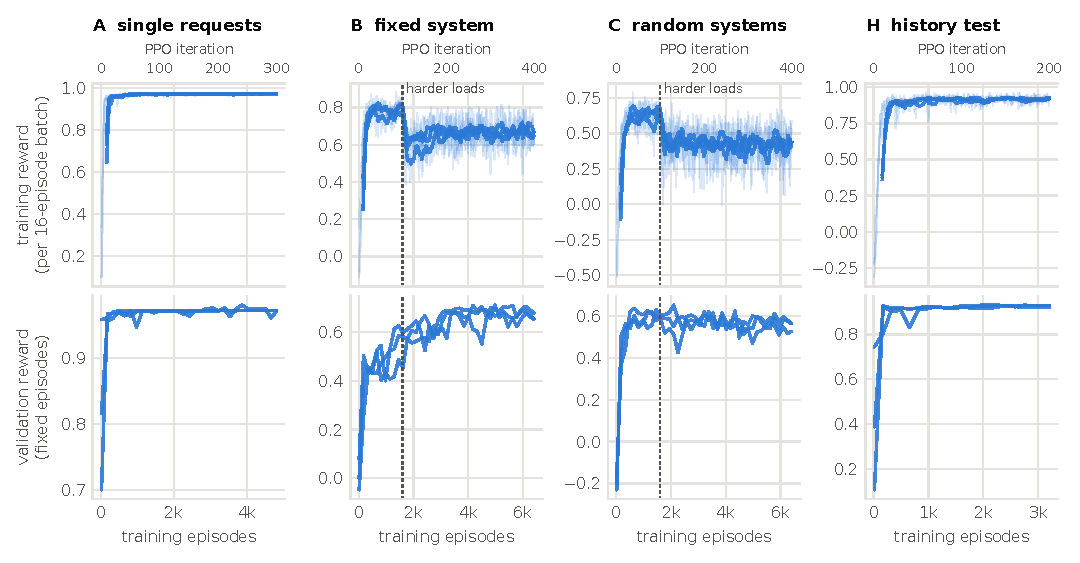
\includegraphics[width=\textwidth]{figures/fig_training.pdf}
\caption{Convergence against the number of training episodes (3 seeds per stage; one line per seed). The top axis shows the matching PPO iteration (1 iteration = 16 episodes). \emph{Top row:} training reward, i.e.\ the mean reward per request of each batch of 16 training episodes (faint) and its moving average over 160 episodes (solid). \emph{Bottom row:} reward on the fixed validation episodes, measured every 160 training episodes. In every stage the reward rises and then flattens, and the three seeds end close together. In B and C the training episodes switch to a wider, harder range of loads after the first quarter (dashed line, a planned curriculum), so the training reward steps down there; the validation episodes do not change, and their reward keeps rising or stays flat.}\label{fig:training}
\end{figure}
\begin{figure}[H]
\centering
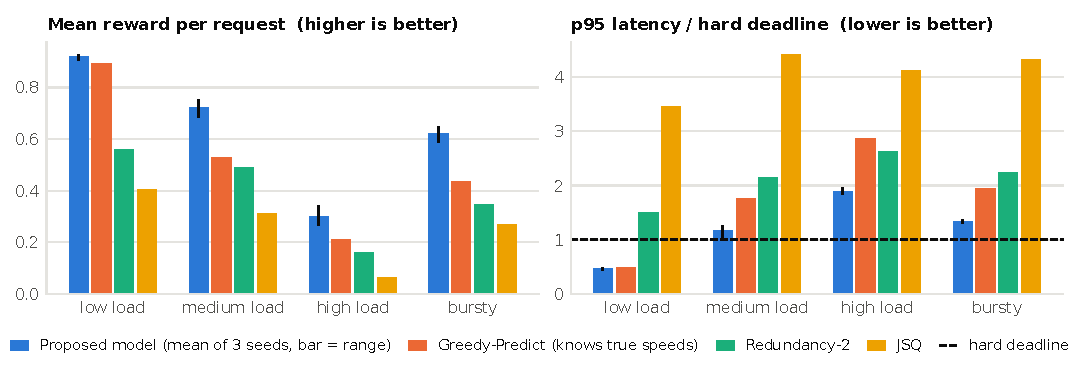
\includegraphics[width=\textwidth]{figures/fig_stageB.pdf}
\caption{Stage B test set. The proposed model (average of 3 seeds; the bar shows the range) compared with the baselines at every load.}
\end{figure}
\begin{figure}[H]
\centering
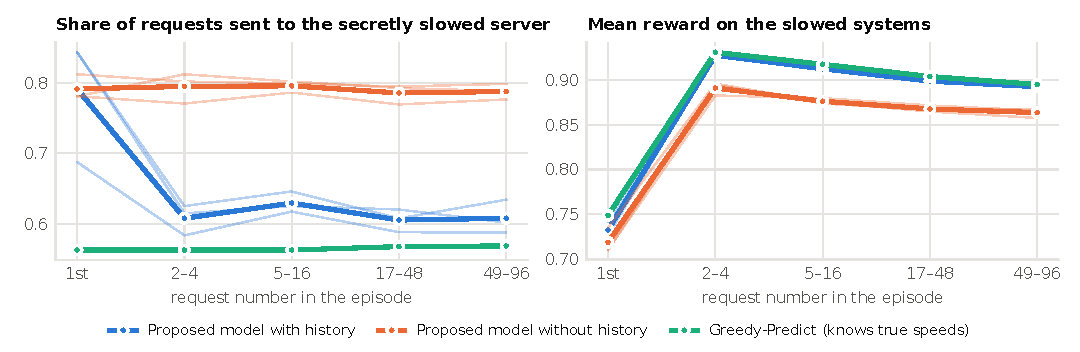
\includegraphics[width=\textwidth]{figures/fig_history.pdf}
\caption{History test H, systems with a slowed server. With history, the model sends less traffic to the slowed server
soon after the first results come back (thin lines = individual seeds). Without history it has no way to notice, so its
traffic does not change. With history, the reward comes close to that of privileged Greedy.}
\end{figure}

\section{What went wrong along the way, and why}\label{sec:failed}
The first runs did not pass every check. The problems below are the ones that taught something about the method itself; each was diagnosed, and its fix was tested before it was kept. The fixes led to the training changes in Section~\ref{sec:changes}. Ordinary coding bugs and adjustments to the test setup were also fixed along the way, but are not listed here.

\begingroup\small
\begin{tabularx}{\textwidth}{@{}P{3.6cm}LL@{}}
\toprule
\hdr{Problem} & \hdr{Cause (found by diagnosis)} & \hdr{Fix and evidence}\\\midrule
Stage A far from the best decisions (first runs: 0\%, 45\% and 69\% within 1\%) & In Stage A each request is independent. But the discounted return mixed the rewards of later, unrelated requests into each decision's credit, which made the learning signal noisy & Give each decision only its own request's reward ($\Delta\to0$) and train for 300 iterations: 99.4\% on every seed (Change~2). Changing only the entropy weight or $\lambda$ did not help (2--52\%)\\
Stage C: history made no difference & (1) In open loop the current state already reveals a slow server, because its running copies take longer, so history adds nothing new. (2) With up to 3 copies per request, it is cheaper to send extra copies than to find the slow server & Added test H, where only history can help. Added the auxiliary speed loss (Change~1). With $\Delta=5$\,ms, history now gives clear gains in closed loop (Section~\ref{sec:results})\\
Test H: history only weakly used without the auxiliary loss & The reward alone is too weak a signal to teach the model to read server speeds from the history & With the auxiliary loss, the traffic share to the slowed server falls from 0.84 to 0.60 (0.79 on the twin where it is not slowed). Without it, the models with and without history score about the same (0.922--0.924 vs 0.910--0.923) (Change~1)\\
Drops late in training, and the ``best'' checkpoint chosen by noise & A constant learning rate is too large late in training, and the validation set was small & Lower the learning rate linearly to $10^{-4}$, and report the model at the end of training (Changes~3 and~5)\\
$\Delta=20$\,ms: B and C lag, and one seed is below Greedy under overload & The return looks about 2\,s ahead, much longer than a request's life ($D^2$ = 150\,ms), so credit is spread over many later requests & With $\Delta=5$\,ms (about 0.5\,s ahead): B and C rewards rise, the C history gain becomes clear in closed loop, and every seed beats Greedy under overload (Change~2)\\
\bottomrule
\end{tabularx}
\endgroup

\section{Required training changes (all tried)}\label{sec:changes}
\begin{goodbox}
\textbf{Scope: training and hyperparameters only.} All five changes concern only \emph{how the model is trained} and \emph{how results are reported}. The conceptual part of the method stays exactly as in the documentation: the problem formulation, the reward and deadlines, the hard rules, the proposed model architecture (token encoder, edge-by-edge decoder with STOP, masks), meta-RL with PPO, and the A\,$\to$\,B\,$\to$\,C training plan. At deployment the model makes decisions exactly as documented; the only addition, the auxiliary speed head, is used during training only.
\end{goodbox}
These five changes are needed for the method to pass. Each one was tried against the documented setting.

\begingroup\small
\begin{tabularx}{\textwidth}{@{}P{4.4cm}P{3.3cm}L@{}}
\toprule
\hdr{Change} & \hdr{Documentation $\to$ new} & \hdr{Why, and the evidence}\\\midrule
1. Auxiliary speed-prediction loss, used during training only: from its internal view of each server, the model also predicts that server's (log) speed. Weight 0.5. The speed is only a training target, never an input & none $\to$ added & Without it, history is hardly used (test H: no clear gain). With it, history gives a clear gain on every seed, and the slowed server is found after the first results. Nothing changes at deployment; the emulator knows the true speeds for training\\
2. Time unit $\Delta$ of the discount (training only) & 100\,ms $\to$ 5\,ms & Each decision looks about $100\,\Delta$ ahead (Section~\ref{sec:data}). With 100\,ms that is about 10\,s, roughly 70 hard deadlines, so the credit of one decision is mixed with the rewards of many unrelated later requests; 5\,ms looks about 0.5\,s ahead, enough to see the effect on the next few requests. 20\,ms was also tested and is worse on average than 5\,ms on B, C and generalisation. Where decisions are independent (Stage A), $\Delta\to0$\\
3. Learning-rate schedule & $3\cdot10^{-4}$ constant $\to$ $10^{-3}$, lowered linearly to $10^{-4}$ & In an early pilot (Stage A, one seed, 40 iterations), the documented settings reached a validation reward of 0.90 vs 0.96 with the tuned settings; that pilot changed the learning rate, $\Delta$, $\lambda$ and minibatch size together. A constant $10^{-3}$ then caused late drops; with the decay the curves flatten and the seeds agree\\
4. Starting bias of the STOP choice & 0 $\to$ +0.5 & The model starts by sending fewer copies, which avoids a wasteful early phase of sending copies everywhere\\
5. How results are reported & --- $\to$ end of training, 3 seeds & Picking the best checkpoint on a small validation set gave misleading numbers (Stage A, seed 0: ``best'' 98.1\% vs end of training 99.4\%)\\
\bottomrule
\end{tabularx}
\endgroup
{\small Three settings were kept from this check but not compared one by one with the documented values: model size $d=64$ with 2
layers (documentation: 128 with 3), $\lambda=0.9$ (documentation: 0.95) and minibatch 256 (documentation: 512). The implementation in the emulator should start from the
configuration that passed here.}

\textbf{Changes to the testing method} (not to the method itself). These were added to make the verdict trustworthy.
\begin{itemize}
\item \textbf{History test H} (closed loop, one copy per request), where only history can reveal which server is slow.
\item \textbf{Paired bootstrap intervals} on twin systems, instead of fixed thresholds.
\item \textbf{Critic target in Stage A.} A single request's reward is mostly random noise, so even a perfect critic can explain at most 12\% of its variance (measured). The documented target of 0.3 is therefore impossible in Stage A. The target used there is half of that maximum, and the critic reaches 75--93\% of the maximum.
\item \textbf{Entropy collapsing too early} is defined as entropy reaching about 0 before the reward has stopped improving. In test H the best policy is fully deterministic, so a low final entropy is correct there.
\item \textbf{Audits.} Every evaluation decision is checked against the hard rules, and the simulator has 12 unit tests.
\end{itemize}

\section{Open points for the emulator stage}\label{sec:open}
\begin{itemize}
\item \textbf{The history comparison must be done in closed loop.} In open loop, queues form, and the running copies already show which server is slow. So the models with and without history score about the same there (Stage C: 0.42--0.47 vs 0.45--0.47), and both avoid the slowed server. In the emulator, the with/without-history comparison should also be run in closed loop (as in test H), and with real slowdowns.
\item \textbf{Only synthetic delays were used.} The next step is the emulator with the measured latency distributions. Stages A--C should be re-run there with the same pass/fail criteria.
\item \textbf{Model size.} Only the small model ($d$=64, 2 layers) was trained. A larger model is needed only if the emulator shows the small one is not enough (the documented size still decides in 1.8\,ms).
\end{itemize}

\section{Final verdict}
\begin{goodbox}
\textbf{Yes, the project is ready to start the implementation in the emulator.} On synthetic data, the method (the proposed model trained with
meta-RL and PPO) converges and does what the design needs:
\begin{itemize}
\item it learns near-optimal decisions;
\item it beats strong baselines, including one that knows the true server speeds;
\item it works on new systems and under changed conditions;
\item it uses its history to adapt to slow servers;
\item it never breaks the hard rules, and it is fast.
\end{itemize}
The emulator implementation should include the five training changes of Section~\ref{sec:changes}, start from the configuration
that passed here, and keep these checks as regression tests for the emulator stage.
\end{goodbox}
\end{document}
